\section{保证与计算成本}
\label{sec:nlipm-guarantees}

第~\ref{chap:lp-interior-point}章证明了线性规划上短步路径跟踪的迭代界。这就需要回答：这个结果在什么条件下能够推广，在什么情形下必须退回局部结论，以及每一轮实际要花多少计算？

\paragraph{为什么要有一个比光滑更强的条件}
Newton法的通常分析用Hessian的Lipschitz常数$M$，结论依赖坐标的选取。障碍函数在边界附近的三阶导数趋于无穷，$M$根本不存在一个有限的整体值。路径跟踪的分析需要一种随点变化的尺子。

用$\phi$自己的Hessian当尺子。下面的条件要求三阶导数被二阶导数控制，这就是\term{自协调}（self-concordant）。

\begin{definition}[自协调障碍]
\label{def:nlipm-self-concordant}
设$\phi$是开凸集上三阶连续可微的凸函数，在边界附近趋于$+\infty$。记$\phi'$、$\phi''$、$\phi'''$为沿方向$\bm{d}$的方向导数。若对所有点和所有方向，
\begin{equation}
 \lvert\phi'''\rvert\leq2(\phi'')^{3/2},\qquad(\phi')^2\leq\vartheta\,\phi'',
 \label{eq:nlipm-self-concordant}
\end{equation}
就称$\phi$是参数为$\vartheta$的自协调障碍。
\end{definition}

对$\phi(x)=-\log x$，沿$d=1$的三个导数是$-1/x$、$1/x^2$、$-2/x^3$。代入两个不等式，都恰好取等号，其中$\vartheta=1$。第一个不等式的两边在缩放$x$时变化相同，所以这个条件不依赖坐标的单位。

三种基本的障碍都是自协调的：$m$条线性约束的对数障碍参数是$m$，二阶锥障碍参数是$2$，$n\times n$半正定锥障碍参数是$n$。凸二次约束的$-\log(-g)$也是自协调的，参数是$1$，所以贯穿例的障碍参数是$\vartheta=2$。

\paragraph{Dikin椭球：局部模型信多远}
自协调的直接后果是，以$\nabla^2\phi$定义的单位椭球落在定义域内：
\begin{equation}
 \bigl\{\bm{x}+\bm{d}:\bm{d}^\top\nabla^2\phi(\bm{x})\bm{d}<1\bigr\}\subset\operatorname{dom}\phi.
 \label{eq:nlipm-dikin}
\end{equation}
这个集合称为\term{Dikin椭球}（Dikin ellipsoid）。多面体的情形可以直接验证：$\bm{g}(\bm{x})=\bm{A}\bm{x}-\bm{b}$时，二次型等于$\sum_i(\bm{a}_i^\top\bm{d}/s_i)^2$。它小于$1$，就有每个$\lvert\bm{a}_i^\top\bm{d}\rvert<s_i$，于是新点的每个松弛都还是正的。

一般情形的证明需要沿线段积分第一个不等式，读者可查阅专著\scite{math-boyd2004convex}。

图~\ref{fig:nlipm-dikin}画出贯穿例的四个Dikin椭球，在椭球边界上逐点计算，松弛都是正的。靠近边界时椭球在法向变扁，在切向仍然较长。这就是局部模型“信多远”的答案，随位置自动调整，不需要知道全局的光滑常数。

\begin{BookInlineFigure}
  \centering
  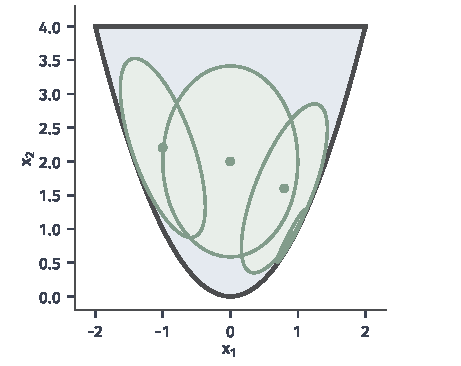
\includegraphics[width=78mm]{figures/05-optimization/06-constrained-optimization/matplotlib/nlipm-dikin/figure.pdf}
  \caption{贯穿例的Dikin椭球，绿点是四个基点，绿色曲线是$\bm{d}^\top\nabla^2\phi(\bm{x})\bm{d}=1$围成的椭球。四个椭球都留在可行集（浅蓝）之内，靠近边界的椭球更扁。}
  \label{fig:nlipm-dikin}
\end{BookInlineFigure}

\paragraph{凸问题的迭代界}
有了这把尺子，第~\ref{chap:lp-interior-point}章的短步分析可以整体推广，其中$\sqrt{n}$换成$\sqrt{\vartheta}$。结论如下，证明要用到自协调函数的Newton减量分析，篇幅较长，读者可查阅专著\scite{math-boyd2004convex}。

\begin{theorem}[路径跟踪的迭代次数]
\label{thm:nlipm-complexity}
设目标是线性函数，可行集有界且有严格可行点，$\phi$是参数为$\vartheta$的自协调障碍，起点足够靠近路径。则短步路径跟踪得到$\varepsilon$精度的解所需的Newton步数为
\begin{equation}
 O\Bigl(\sqrt{\vartheta}\,\log\frac{\vartheta\mu^{(0)}}{\varepsilon}\Bigr).
 \label{eq:nlipm-complexity}
\end{equation}
\end{theorem}

这个界不依赖$f$和$g_i$的条件数，只依赖$\vartheta$，这是内点法在凸问题上最强的结论。目标非线性时，可以用上图形式把它移进约束，代价是要为新的约束找到自协调障碍。

式~\eqref{eq:nlipm-complexity}也解释了为什么锥结构有价值。一个$q+1$维的二阶锥只贡献$\vartheta=2$，如果把它拆成很多线性不等式去逼近，$\vartheta$就随拆分的条数增长。

\paragraph{线性规划的结论不能外推}
多项式界依赖两件事：约束有容易计算的自协调障碍，并且问题是凸的。两者都可能不成立。

第一，凸性并不自动给出自协调。取$g(x)=\mathrm{e}^x-1\leq0$，障碍$\phi=-\log(1-\mathrm{e}^x)$是凸函数，但$x\to-\infty$时$\phi''$和$\phi'''$都约等于$\mathrm{e}^x$，于是
\[
 \frac{\lvert\phi'''\rvert}{(\phi'')^{3/2}}\approx\mathrm{e}^{-x/2}\to\infty.
\]
第一个不等式不可能成立。每个开凸集都存在参数为$O(n)$的自协调障碍，但这是存在性的结果，这样的障碍一般无法计算。

第二，非凸问题求全局解是NP难的，非凸二次规划就已经如此，所以不可能有类似式~\eqref{eq:nlipm-complexity}的全局结果，除非$\mathrm{P}=\mathrm{NP}$。

\paragraph{非凸问题的局部收敛}
非凸问题上能证明的是：在定理~\ref{thm:nlipm-local-path}的条件下，从足够近的点出发，Newton迭代跟着路径收敛到KKT点。下面给出一步的估计。记$\bm{z}^\star$为该KKT点及其松弛、乘子，$\bm{F}_\mu(\bm{z})=\bm{F}_0(\bm{z})-\mu\bm{e}$，其中$\bm{e}$只在互补方程处为$1$，$\bm{G}$是$\bm{F}_0$的Jacobian矩阵。

\begin{theorem}[Newton步的局部估计]
\label{thm:nlipm-local-rate}
设定理~\ref{thm:nlipm-local-path}的条件成立，$\nabla^2f$、$\nabla^2g_i$、$\nabla^2h_j$在$\bm{x}^\star$附近是$M$-Lipschitz的。则存在$\bm{z}^\star$的邻域和常数$C_{\mathrm{G}}$、$M_{\mathrm{G}}$、$C_{\mathrm{p}}$（$M_{\mathrm{G}}$由$M$和乘子的界决定），使邻域内的$\bm{z}$和足够小的$\mu^+>0$满足：单位Newton步
\begin{equation}
 \bm{z}^+=\bm{z}-\bm{G}(\bm{z})^{-1}\bm{F}_{\mu^+}(\bm{z})
 \label{eq:nlipm-local-step}
\end{equation}
有
\begin{equation}
 \lVert\bm{z}^+-\bm{z}^\star\rVert_2\leq\frac{C_{\mathrm{G}}M_{\mathrm{G}}}{2}\bigl(\lVert\bm{z}-\bm{z}^\star\rVert_2+C_{\mathrm{p}}\mu^+\bigr)^2+C_{\mathrm{p}}\mu^+.
 \label{eq:nlipm-local-rate}
\end{equation}
\end{theorem}

\begin{proof}
定理~\ref{thm:nlipm-local-path}的证明说明$\bm{G}(\bm{z}^\star)$非奇异，所以在邻域内
\[
 \lVert\bm{G}(\bm{z})^{-1}\rVert_2\leq C_{\mathrm{G}}.
\]
$\bm{G}$的各块由$\nabla f$、$\nabla^2f$、$\nabla^2g_i$、$\nabla^2h_j$和乘子组成，因此在邻域内是$M_{\mathrm{G}}$-Lipschitz的。路径连续可微，所以
\[
 \lVert\bm{z}(\mu)-\bm{z}^\star\rVert_2\leq C_{\mathrm{p}}\mu.
\]

记$\bm{z}'=\bm{z}(\mu^+)$，它满足$\bm{F}_{\mu^+}(\bm{z}')=\bm{0}$。由Newton步的定义，
\[
 \bm{z}^+-\bm{z}'=\bm{G}(\bm{z})^{-1}\Bigl[\bm{G}(\bm{z})(\bm{z}-\bm{z}')-\bigl(\bm{F}_{\mu^+}(\bm{z})-\bm{F}_{\mu^+}(\bm{z}')\bigr)\Bigr].
\]
方括号内是一阶Taylor余项，由$\bm{G}$的Lipschitz性，它的范数不超过$\tfrac12M_{\mathrm{G}}\lVert\bm{z}-\bm{z}'\rVert_2^2$。于是
\[
 \lVert\bm{z}^+-\bm{z}'\rVert_2\leq\tfrac12C_{\mathrm{G}}M_{\mathrm{G}}\lVert\bm{z}-\bm{z}'\rVert_2^2.
\]
由三角不等式，$\bm{z}$到$\bm{z}'$的距离满足
\[
 \lVert\bm{z}-\bm{z}'\rVert_2\leq\lVert\bm{z}-\bm{z}^\star\rVert_2+C_{\mathrm{p}}\mu^+.
\]
再对$\bm{z}^+$用一次三角不等式，即得结论。
\end{proof}

式~\eqref{eq:nlipm-local-rate}右端有两项：Newton法自身的二次项，以及目标参数的偏移。$\mu^+$与当前误差同阶时，收敛是线性的，表~\ref{tab:nlipm-run}中$\sigma$固定为$0.2$，误差每轮大约乘以$0.2$，就是这种情形。按式~\eqref{eq:nlipm-mu-update}让$\mu^+$超线性减小，收敛速度也变成超线性。

这个估计假设单位步可以走，定理本身没有保证这一点，还要证明$\alpha=1$满足比例规则：活动约束的$s_i$和不活动约束的$\lambda_i$都是$O(\mu)$量级的小量，方向也必须是相应量级，这需要参数更新不能太快，也需要$\eta\to1$。完整的论证较长，读者可查阅专著\scite{math-nocedal2006numerical}。

\paragraph{全局的情形}
从任意点出发，非凸问题上能证明的是：在迭代点有界、矩阵经过惯性修正、约束正则等假设下，带过滤器或合成目标检验的算法的极限点要么满足KKT条件，要么是约束违反量的驻点。这里没有全局最优的保证，图~\ref{fig:nlipm-nonconvex-fold}已经说明，路径本身可能走向较差的局部解。表~\ref{tab:nlipm-claims}总结了两类问题上结论的区别。

\begin{BookInlineTable}
  \centering
  \footnotesize
  \begin{tabular}{@{}lll@{}}
    \toprule
    问题 & 凸问题 & 一般非凸问题\\
    \midrule
    路径 & 整条存在且唯一 & 只在KKT点附近\\
    路径上的间隙 & $f-f^\star\leq m\mu$ & 无全局含义\\
    迭代界 & 自协调时$\sqrt{\vartheta}$型 & 无\\
    停止的含义 & 近似全局解的证书 & 近似KKT点\\
    不可行的判定 & 可给证书 & 只能报告局部驻点\\
    局部速度 & 超线性 & 正则性下超线性\\
    \bottomrule
  \end{tabular}
  \caption{内点法在凸问题与非凸问题上的结论。}
  \label{tab:nlipm-claims}
\end{BookInlineTable}

\paragraph{每一轮的代价}
一轮的工作分三块：计算$f$、$\bm{g}$、$\bm{h}$及其一二阶导数，分解线性系统，以及可能的回溯。回溯只重新计算函数值，比较便宜。决定性的是分解。

压缩矩阵$\tilde{\bm{H}}=\bm{W}+\bm{J}^\top\bm{D}\bm{J}$是$n\times n$的。若有一条约束涉及很多变量，$\bm{J}$有一个稠密的行，$\bm{J}^\top\bm{D}\bm{J}$就是稠密的。鞍点形式~\eqref{eq:nlipm-saddle}维数大，却保留了稀疏性。

图~\ref{fig:nlipm-sparse-fill}是一个$n=m=20$的算例，$\bm{J}$是双对角的，最后一行稠密，共$58$个非零元，取$\bm{W}=\bm{I}$。压缩矩阵完全稠密，它的下三角因子有$210$个非零元。$40\times40$的鞍点矩阵把稠密行排在最后，下三角因子只有$117$个非零元。

这和第~\ref{chap:lp-interior-point}章的$\bm{A}\bm{D}\bm{A}^\top$是同一个现象，只是这里还多了$\bm{W}$。稠密情形下，$n\times n$的分解需要约$n^3/3$次运算；鞍点矩阵不定，要用$\bm{L}\bm{D}\bm{L}^\top$分解和主元选择，主元顺序会随数值改变，符号分析不能像线性规划那样只做一次。每试一个$\delta_{\mathrm{w}}$就要重新分解一次。

\begin{BookInlineFigure}
  \centering
  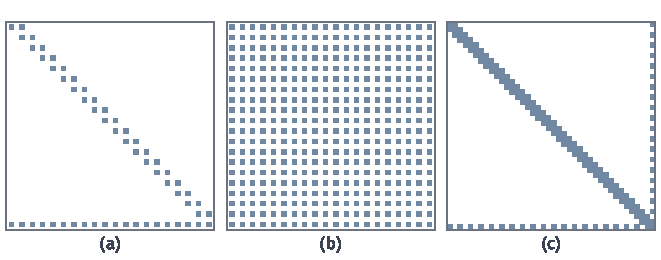
\includegraphics[width=112mm]{figures/05-optimization/06-constrained-optimization/matplotlib/nlipm-sparse-fill/figure.pdf}
  \caption{三个矩阵的非零模式，蓝点表示非零元。(a)$20\times20$的Jacobian矩阵，双对角加上一个稠密行。(b)压缩矩阵$\bm{W}+\bm{J}^\top\bm{D}\bm{J}$，完全稠密。(c)鞍点矩阵$[\bm{W},\bm{J}^\top;\bm{J},-\bm{D}^{-1}]$，变量与约束交错排列，稠密行排在最后。}
  \label{fig:nlipm-sparse-fill}
\end{BookInlineFigure}

\paragraph{条件数}
$\bm{D}$的对角元是$\lambda_i/s_i$。$\mu\to0$时，活动约束上它约为$(\lambda_i^\star)^2/\mu$，趋于无穷，不活动约束上它约为$\mu/(s_i^\star)^2$，趋于零，矩阵的条件数按$1/\mu$增长。

图~\ref{fig:nlipm-cond-growth}显示，贯穿例的压缩矩阵和鞍点矩阵都是如此，保留鞍点结构并不能消除这种病态，它的好处在稀疏性。这种病态的结构很特殊，向后稳定的直接分解能够得到足够准确的方向；迭代法就没有这样幸运，共轭梯度类的方法在$\mu$小时需要专门的预条件子。

\begin{BookInlineFigure}
  \centering
  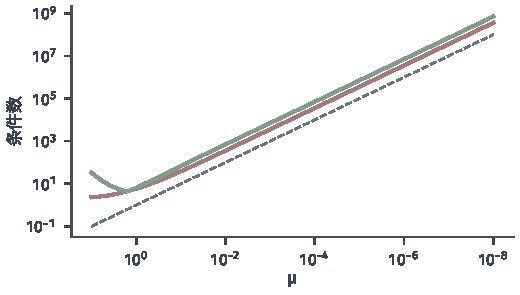
\includegraphics[width=88mm]{figures/05-optimization/06-constrained-optimization/matplotlib/nlipm-cond-growth/figure.pdf}
  \caption{贯穿例沿中心路径的条件数，横轴是$\mu$，向右减小。红线是压缩矩阵$\tilde{\bm{H}}$，绿线是鞍点矩阵，灰色虚线是参照线$1/\mu$。两条曲线都按$1/\mu$增长。}
  \label{fig:nlipm-cond-growth}
\end{BookInlineFigure}

\paragraph{外层轮数}
总代价等于外层轮数乘以每轮的分解代价。实际问题上，原始—对偶方法通常几十轮结束，这是经验而不是定理，它在式~\eqref{eq:nlipm-complexity}的界之下很多。

与第~\ref{chap:feasible-iterations}章的可行迭代和第~\ref{chap:penalty-multiplier-methods}章的乘子方法相比，内点法每轮的代价高，轮数少。能够精确分解时，内点法很有优势；分解太贵、只能得到低精度解就够时，一阶方法更合适。
